\section{Solution analysis}
After a high level discussion about the characteristics of the solution proposed by this work, now it is time to make an additional step in the road that leads to the concretization of a working system that realizes such idea.

Here, the Domain will be explored, clarifying concepts and nomenclatures in order to uniquely identify the building blocks needed to move forward.
Then, use cases will be discussed, explaining what the system needs to do, seen from the point of view of the actors interacting with it.
Finally, the requirements will be presented, aiming to provide a clear set of criteria to satisfy for a system that wants to use the Transparent scheduling model over heterogeneous devices.

\subsection{Domain}
TODO

\subsection{Use cases}
TODO

%\begin{figure}[!ht]
    %\centering
    %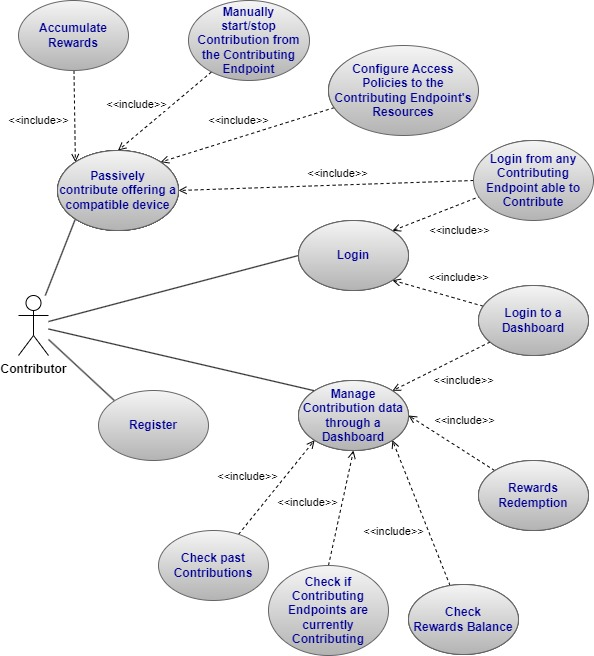
\includegraphics[width=\linewidth]{document/chapters/chapter_5/images/contributor_use_cases.jpg}
    %\caption{Contributor's use cases diagram}
    %\label{fig:use_cases_contributor}
%\end{figure}

%\begin{figure}[!ht]
    %\centering
    %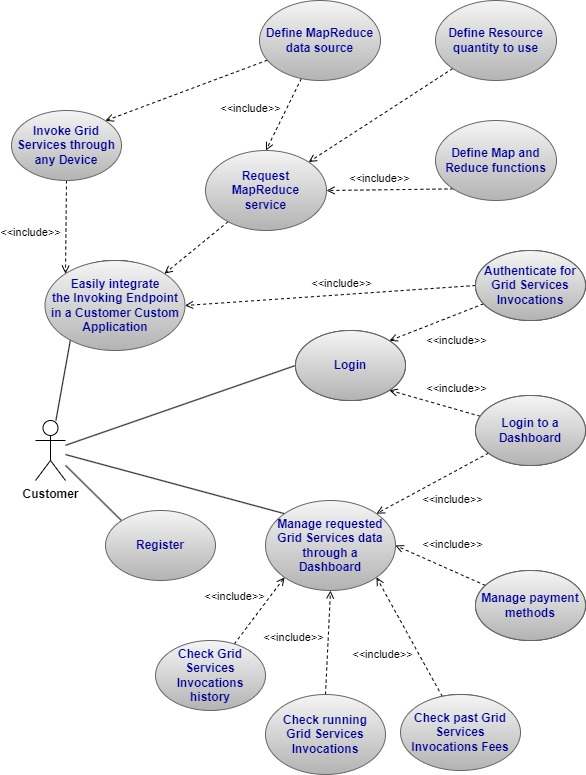
\includegraphics[width=\linewidth]{document/chapters/chapter_5/images/customer_use_cases.jpg}
    %\caption{Customer's use cases diagram}
    %\label{fig:use_cases_customer}
%\end{figure}

\subsection{Requirements}
TODO

\subsubsection{Must have}
All the requirements that are necessary for the successful completion of a complete production release.

\paragraph{Contributor side}
\begin{itemize}
    \item \textbf{Registration and identification}
    \begin{itemize}
        \item The Contributor must be able to register to the Grid system in order to uniquely identify contributions regarding its devices participating in the Grid.
        \item Once authenticated to a contributing device, the Contributor must not be requested to authenticate again unless it is absolutely necessary.
    \end{itemize}
    \item \textbf{Contribution}
    \begin{itemize}
        \item It must be possible to contribute to the Grid using any device among Computers, Smartphones and Tablets running the most popular respective Operative Systems.
        \item Configuration for the Contributor must be easy, guided and fast (5 minutes maximum).
        \item Every device that the Contributor offers must be configured just once and require no additional efforts unless the Contributor chooses to change configurations.
    \end{itemize}
    \item \textbf{Rewards}
    \begin{itemize}
        \item Every successful contribution to the execution of a Grid service must be registered contributing to the rewards balance of the Contributor.
        \item The Contributor must be able to see its current rewards balance.
        \item The Contributor must be able to see past contributions in which its devices contributed to the execution of a certain Grid service.
        \item Once a certain monetary threshold is reached, the Customer must be able to withdraw its rewards from its balance.
    \end{itemize}
    \item \textbf{Security}
    \begin{itemize}
        \item Execution environment-specific security measures must be implemented to protect the Contributor.
    \end{itemize}
    \item \textbf{User experience}
    \begin{itemize}
        \item The application running on mobile devices (used to contribute to the Grid) must be aware of battery status in order not to drain battery in low-battery situations.
        \item The application running on mobile devices (used to contribute to the Grid) must be aware of the type of connection used in order not to drain data from the Consumer mobile plan (unless the Consumer allows this possibility).
    \end{itemize}
\end{itemize}
\paragraph{Customer side}
\begin{itemize}
    \item \textbf{Registration and identification}
    \begin{itemize}
        \item The Customer must be able to register to access Grid's services.
        \item The Customer must go through a verification process in order to be reliable and accountable before being able to use Grid's services.
    \end{itemize}
    \item \textbf{Payments}
    \begin{itemize}
        \item The Customer must be able to register its payment method once and use it every time it invokes one Grid's service.
        \item The Customer must pay individual Grid's services invocations.
    \end{itemize}
    \item \textbf{Framework utilization}
    \begin{itemize}
        \item The Customer must be able to integrate the Framework in its own project to utilize the Grid's services.
        \item The Customer must be able to invoke Grid’s services from any adequate device (Computer, Tablet or Smartphone) using the integrated Framework.
        \item The Customer must be able to easily increase/decrease the amount of Grid's resources tapped into, removing the underlying complexity.
    \end{itemize}
    \item \textbf{MapReduce service utilization}
    \begin{itemize}
        \item The Customer must be able to implement its own Map and Reduce functions in a MapReduce service invocation.
        \item The MapReduce parameters such as number of Map and Reduce workers must be configurable by the Customer.
        \item The Customer must be able to define the data source for the MapReduce execution (whether from the invoking device or an external source).
    \end{itemize}
\end{itemize}
\paragraph{Project side}
\begin{itemize}
    \item \textbf{Scalability}
    \begin{itemize}
        \item The Grid system must be able to easily scale horizontally in a fully automated way.
        \item Grid backend services must be as loosely coupled as possible, resulting in a modular composition of technologically independent services that operate exchanging messages over defined channels.
        \item It must be possible to create on the go (depending on needs dictated by the current traffic) multiple instances of the Grid backend services, employing a mechanism to discover and contact such new instances.
    \end{itemize}
    \item \textbf{Efficiency}
    \begin{itemize}
        \item Employed resources for running the Grid system must be adequate to the load that the system has to currently handle, dynamically adjusting to cut expenses.
        \item The Grid system must be geographically-aware and manage node utilization taking in account physical distance in order to reduce latency, improving performances.
        \item When possible, services must be implemented in a way that reduces traffic to the Grid’s systems, moving such traffic to the contributing Nodes.
        \item Every execution of a service offered by the Grid must use Nodes that have sufficient capabilities to complete the task adequately.
    \end{itemize}
    \item \textbf{Compatibility}
    \begin{itemize}
        \item The Framework developed for Customers and the Core of the Contribution application for Contributors must be implemented using a technology that can be easily integrated in all major Operative Systems that run on the target devices.
    \end{itemize}
    \item \textbf{MapReduce}
    \begin{itemize}
        \item The MapReduce execution must grant an adequate level of reliability and fault tolerance.
        \item The MapReduce tasks on the Node side must be designed in a way that allows to integrate support for new programming  languages for the execution of Customer-defined Map and Reduce functions.
    \end{itemize}
    \item \textbf{Expandability and maintainability}
    \begin{itemize}
        \item The solution must be designed in a way that allows to easily expand the capabilities of the Grid, allowing the creation of newer services that can be executed using the Nodes.
        \item It must be possible to parallelize implementation of features and maintenance, structuring the solution using a microservices approach allowing multiple teams to work on multiple sub-portions of the project.
    \end{itemize}
    \item \textbf{Security}
    \begin{itemize}
        \item Communications between the components of the Grid must be cyphered and use other security measures.
        \item There must be a permission system used to manage access to a Node resource.
        \item Operations inside the Grid must be logged in order to have a fully comprehensive view of every movement that happens inside the system.
    \end{itemize}
\end{itemize}

\subsubsection{Should have}
Requirements that are important but not necessary for a production release and can be postponed to subsequent releases.

\paragraph{Contributor side}
\begin{itemize}
    \item It should be possible to see the status of every device owned by the Contributor.
    \item It should be possible, from the contributing device, to see the local current status.
    \item It should be possible to limit the access to certain resources of the device.
    \item It should be possible to manually enable/disable the contribution of a device.
    \item It should be possible to schedule a trigger (time and/or events) to start/stop the contribution.
    \item The applications used by the Contributors should limit usage of resources if the user is actively using the device in order to not have a negative impact on user experience (avoiding incentives for the user to uninstall the application).
\end{itemize}
\paragraph{Customer side}
\begin{itemize}
    \item There should be a tool for testing the Map and Reduce functions.
    \item It should be possible to specify the minimum capabilities of the devices involved in the execution of a Grid service.
\end{itemize}
\paragraph{Project side}
\begin{itemize}
    \item There should be device-specific optimizations.
\end{itemize}

\subsubsection{Could have}
Requirements that are nice to have but have a much smaller impact when left out of the release.
\paragraph{Customer side}
\begin{itemize}
    \item There could be a standardized MapReduce web tool that enables less specialized organizations (from a technological point of view) to perform operations constructed by a facilitated GUI.
\end{itemize}